\documentclass[conference]{IEEEtran}
\IEEEoverridecommandlockouts
\usepackage{cite}
\usepackage{amsmath,amssymb,amsfonts}
\usepackage{graphicx}
\usepackage{booktabs}
\usepackage{array}
\usepackage{url}
\graphicspath{{./plots/}}

\begin{document}

\title{When Does the Knowledge Graph Help?\\
Question-Driven Retrieval Routing for EHR-Grounded Clinical Question Answering}

\author{
\IEEEauthorblockN{[AUTHOR NAME]}
\IEEEauthorblockA{
\textit{[AFFILIATION],}\\
[UNIVERSITY], [CITY, COUNTRY]\\
[EMAIL]
}
}

\maketitle

\begin{abstract}
Hybrid clinical retrieval-augmented generation~(RAG) systems commonly
apply every retrieval source---note search, structured electronic
health record~(EHR) lookup, and knowledge graph~(KG) traversal---to
every question, which is costly and may be unnecessary. We ask whether
a learned router selecting among text only~(T), text with an EHR
snapshot~(T+E), and text with EHR and KG facts~(T+E+K) can match
always-on hybrid retrieval at lower cost, and when KG augmentation
helps. Our pipeline runs on one consumer GPU (RTX~4050, 6~GB VRAM):
a MIMIC-IV lakehouse, a 25-disease knowledge graph, a FAISS index over
2{,}282{,}927 note chunks, and MedGemma-1.5-4B fine-tuned with QLoRA
on retrieval-augmented prompts. On 300 held-out questions from
patients disjoint from all fine-tuning and router data, the router is
statistically indistinguishable from
always-on hybrid retrieval on BLEU, ROUGE-L, and BERTScore~F1 (all
$p > 0.05$, paired Wilcoxon) while cutting mean latency by 46.8\%
(4005~ms vs.\ 7528~ms), invoking the KG on 17.3\% of questions. Two
pre-registered expectations fail, and we report both. A feature
ablation shows patient-level features contribute nothing to routing
(macro-F1 $-0.018$ versus a question-embedding-only router), making
the system question-driven rather than patient-adaptive.
Under a length-controlled grounding measure the router remains
significantly less grounded than always-on hybrid retrieval ($0.5379$
vs.\ $0.6271$, $p = 1.2\times10^{-5}$)---a real efficiency-grounding
trade-off, not a metric artifact. KG benefit also \textit{decreases}
with EHR sparsity ($+1.95$ vs.\ $+0.57$ BERTScore points in low- and
high-sparsity cases), because KG retrieval is keyed on the diagnosis
list that sparse records lack. Questions are template-generated; the
system is a research prototype without clinical validation.
\end{abstract}

\begin{IEEEkeywords}
adaptive retrieval, retrieval-augmented generation, knowledge graph,
clinical question answering, electronic health records, MIMIC-IV,
QLoRA, parameter-efficient fine-tuning, EHR sparsity, consumer GPU
\end{IEEEkeywords}

\section{Introduction}

Clinical question answering systems increasingly combine several
retrieval sources: free-text search over clinical notes, lookups
against structured EHR tables, and traversal of curated medical
knowledge graphs. The prevailing design applies all available sources
to every question. This is simple to implement and difficult to fault
on quality grounds, but it is not obviously efficient: if a patient's
structured record already contains the information a question asks
for, retrieving and injecting additional knowledge-graph context adds
latency and prompt length without adding evidence.

We study whether that cost is necessary. Concretely, we ask two
questions. \textbf{H1:} can a learned router that selects among three
retrieval configurations---text only~(T), text with a structured EHR
snapshot~(T+E), and text with EHR and knowledge-graph facts
(T+E+K)---preserve the answer quality of always-on hybrid retrieval
while reducing latency and hallucination? \textbf{H2:} does the
benefit of knowledge-graph augmentation depend on how sparse the
patient's structured record is, growing as the EHR provides less?

Answering these questions requires an evaluation design that can
actually distinguish the modes. Two properties matter. First, the
generator must be trained on the same prompt structures it is
evaluated on, otherwise mode differences measure distribution shift
rather than retrieval value. Second, knowledge-graph facts must not
be memorised during fine-tuning, since disease-level clinical facts
are patient-independent and therefore transfer freely across a
patient-level data split. We address both explicitly.

Our contributions are four. First, we present a fully reproducible
adaptive-retrieval pipeline for EHR-grounded clinical QA that runs
end to end on a single 6~GB consumer GPU, in which fine-tuning prompts
are constructed by the same retriever used at inference and every
retrieval mode receives an identical, budgeted passage block so that
modes differ only by the additive presence of EHR and KG content.
Second, we evaluate seven systems on 300 held-out questions and show
that the router matches always-on hybrid retrieval on all three
quality metrics with no statistically detectable difference, at 46.8\%
lower latency, and that it also outperforms a static question-type
routing policy and a random-routing baseline. Third, we report a
feature ablation demonstrating that patient-level structural features
contribute no measurable routing signal, which contradicts the
adaptive-routing framing that motivated the work and reframes the
router as a question-driven policy. Fourth, we show that the standard
word-overlap grounding metric is substantially a proxy for context
length (pooled $r = -0.52$), introduce a length-controlled measure,
and find that the router's grounding deficit survives the correction
and that text-only retrieval is close to entirely ungrounded.

\section{Related Work}

\subsection{Clinical Language Models}

Language models have been applied across a widening range of clinical
tasks, from information extraction to open-ended question answering,
with the reported capabilities and the associated evaluation and
safety concerns surveyed by Thirunavukarasu \textit{et
al.}~\cite{thirunavukarasu2023}. Openly released medically adapted
models are of particular interest for settings where cloud inference
is unattractive on privacy or cost grounds, since they can be run and
adapted locally. We use MedGemma-1.5-4B, an openly released medically
tuned model built on the Gemma~3 family~\cite{medgemma2025}, whose
4-bit quantised footprint fits within a 6~GB VRAM budget.

\subsection{Retrieval-Augmented Generation for Clinical Text}

Retrieval-augmented generation conditions a generator on passages
retrieved from an external corpus, improving factuality on
knowledge-intensive tasks without modifying model
weights~\cite{lewis2020}. Dense retrieval over sentence embeddings is
the standard instantiation~\cite{reimers2019}, typically served by an
approximate nearest-neighbour index~\cite{johnson2019}. In medicine, systematic benchmarking across
corpora, retrievers, and backbone models shows that retrieval can
substantially improve question-answering accuracy but that the gain
depends strongly on the particular combination
used~\cite{xiong2024}. Clinical deployments additionally have access
to a second, patient-specific evidence source---the structured record
of the individual patient---which has no corpus-level analogue. Our
T+E mode corresponds to that configuration.

\subsection{Knowledge-Graph-Augmented Retrieval}

A complementary line of work injects structured relational knowledge
by building a graph over entities and their relations and conditioning
generation on retrieved portions of it, rather than on flat passages
alone~\cite{edge2024}. Our T+E+K mode follows this pattern in a
deliberately simple form: we construct a graph whose nodes are
diseases, symptoms, laboratory tests, and drugs, and retrieve the
one-hop neighbourhood of diseases matched from the patient's diagnosis
list. Section~\ref{sec:mkg} describes the relation types we encode and
how the edges were obtained.

\subsection{Adaptive and Selective Retrieval}

Rather than retrieving unconditionally, adaptive retrieval methods
decide per query whether and how much to retrieve, motivated by both
cost and the observation that unnecessary context can degrade
generation. Self-RAG trains a model to decide when retrieval is
warranted and to critique the passages it
retrieves~\cite{asai2024}, while Adaptive-RAG selects among
no-retrieval, single-step, and multi-step strategies according to an
estimate of question complexity~\cite{jeong2024}. Both vary the
\textit{amount} of retrieval over a single homogeneous corpus. The
multi-source clinical setting differs in kind: the choice is which of
several heterogeneous evidence sources to consult---free text, the
structured patient record, and a knowledge graph---each carrying a
different retrieval cost and a different failure mode.

\subsection{Research Gap}

Two gaps motivate this study. First, multi-source clinical RAG systems
are typically evaluated as fixed always-on configurations, so the
marginal value of the most expensive source---knowledge-graph
traversal---is rarely isolated. Second, where adaptive retrieval is
proposed, it is seldom compared against the trivial baselines that
would falsify it, namely a static per-question-type policy and an
oracle upper bound. We evaluate against both, and we test the
mechanism of our own router by ablation rather than inferring it from
feature-importance scores.

\section{Methodology}

\subsection{Clinical Lakehouse and EHR Sparsity Characterisation}

MIMIC-IV~\cite{mimiciv2023} tables are converted to Parquet and queried
through DuckDB~\cite{duckdb2019}. A \textit{PatientSnapshot} interface
returns, for any admission, its demographics, ordered diagnoses,
laboratory results with abnormality flags, vital signs, and
medications, and renders them as a compact textual snapshot.

To characterise how much structured evidence an admission provides, we
compute a sparsity score $S$ as in~\eqref{eq:sparsity}, combining three
indicators: the number of distinct laboratory tests $n_{\text{labs}}$,
the number of distinct diagnoses $n_{\text{diag}}$, and the interval
$d_{\text{note}}$ in days between the last clinical note and
discharge,

\begin{equation}
\label{eq:sparsity}
\begin{split}
S = \; &\alpha_1 \cdot \mathbb{1}[\,n_{\text{labs}} < \tau_{\text{labs}}\,] \\
     + &\alpha_2 \cdot \mathbb{1}[\,n_{\text{diag}} < \tau_{\text{diag}}\,] \\
     + &\alpha_3 \cdot \mathbb{1}[\,d_{\text{note}} > \tau_{\text{days}}\,],
\end{split}
\end{equation}

with $\alpha_1 = \alpha_2 = \alpha_3 = 1$ and thresholds
$\tau_{\text{labs}} = 5$, $\tau_{\text{diag}} = 3$,
$\tau_{\text{days}} = 7$. Admissions are bucketed as \textit{high}
sparsity ($S \geq 2$), \textit{medium} ($S = 1$), or \textit{low}
($S = 0$). Admissions with no notes receive a sentinel
$d_{\text{note}}$ value and therefore satisfy the third indicator.

\subsection{Medical Knowledge Graph Construction}
\label{sec:mkg}

The knowledge graph covers 25 chronic and acute conditions and is
stored in Neo4j. Guideline-derived edges are hand-curated into four
relation types---\texttt{HAS\_SYMPTOM}, \texttt{INDICATES\_LAB},
\texttt{FIRST\_LINE\_TREATMENT}, and
\texttt{CONTRAINDICATED\_WITH}---giving 215 edges over 51 symptom, 32
laboratory, and 27 drug nodes (Table~\ref{tab:mkg}). A second,
data-driven relation \texttt{CO\_OCCURS\_WITH\_LAB} is computed
directly from MIMIC-IV by measuring, for each seed disease, the
fraction of that disease's admissions in which each laboratory test
appears, retaining tests above a 5\% co-occurrence threshold; this
yields 375 additional edges.

At retrieval time, a patient's diagnosis strings and the question text
are matched against disease node names by non-stopword term overlap,
accepting matches above a fixed overlap threshold, and the one-hop
neighbourhood of each matched disease is linearised into natural
language statements.

\subsection{Retrieval Modes and Context Budgeting}

Clinical notes are chunked and embedded with
BAAI/bge-small-en-v1.5~\cite{bge2024} into a 384-dimensional FAISS
inner-product index of 2{,}282{,}927 vectors, queried at $k = 5$. The
three retrieval modes are strictly additive: T supplies retrieved
passages only; T+E adds the structured EHR snapshot; T+E+K adds
linearised KG facts.

Because these prompts are far longer than the gold answers, we impose
a fixed per-section token budget rather than truncating the assembled
prompt. Passages receive 600 tokens, the EHR snapshot 350, and KG
facts 350, within a total sequence budget of 1524 tokens. Two
properties follow. First, the question and gold answer can never be
truncated away. Second, because the passage budget is identical across
modes, the passage block for a given question is byte-identical in all
three modes, so the modes differ \textit{only} by the additive presence
of EHR and KG content. Passages are dropped lowest-ranked-first when
the budget binds, so surviving evidence is the highest-scoring.

\subsection{Retrieval-Aligned QLoRA Fine-Tuning}

MedGemma-1.5-4B is fine-tuned with QLoRA~\cite{dettmers2023}, applying
low-rank adapters~\cite{hu2022} of rank 16 and $\alpha = 32$ with
dropout 0.10 to all linear projections of a 4-bit NF4-quantised base
model. Training uses \texttt{adamw\_8bit}, learning rate
$2\times10^{-4}$ with cosine decay, batch size 1 with gradient
accumulation 8, gradient checkpointing, and early stopping on
validation loss.

Two design choices are essential to the validity of the comparison.
First, training prompts are constructed by \textit{the same retriever
used at inference}: each example is assigned a retrieval mode
independently and reproducibly, giving 346 T, 339 T+E, and 315 T+E+K
training prompts, so the model is trained on the exact prompt
structures it is later evaluated on. Second, loss is computed on the
completion only. With a mean gold answer of roughly 24 tokens against
contexts of 2000--2600 tokens, computing loss over the full sequence
would place more than 99\% of the gradient signal on reproducing
retrieved context rather than on answering. Training converged to a
best validation loss of 0.3788.

\subsection{Oracle Label Generation and Router Training}

Router supervision is generated by running all three modes on each
router-split question and scoring each output against the reference
with a composite of BERTScore~F1~\cite{zhang2020} (0.60),
ROUGE-L~\cite{lin2004} (0.25), and exact match (0.15), less a penalty
for heuristically detected hallucination. A small ascending cost is subtracted per mode, and the
cheapest mode within a tolerance of the best composite is selected, so
that when additional retrieval yields no measurable quality gain the
label prefers the cheaper configuration. The resulting label
distribution is 118 T+E, 44 T, and 38 T+E+K on router-train, and 59,
23, and 18 respectively on router-validation.

The router is a gradient-boosted decision tree
classifier~\cite{chen2016} over a 389-dimensional feature vector: a
384-dimensional BGE embedding of the question, concatenated with five
structural patient features ($n_{\text{labs}}$, $n_{\text{diag}}$,
$n_{\text{meds}}$, the sparsity score, and the encoded sparsity
bucket). Class weights are balanced and hyperparameters are selected
by randomised search over five stratified folds. Section~\ref{sec:ablation}
ablates this feature set.

\section{Experimental Setup}

\subsection{Hardware and Software}

All experiments run on a single NVIDIA GeForce RTX~4050 Laptop GPU
with 6~GB VRAM under Windows~11, CUDA~12.1, and PyTorch~2.5.1. The
generator is loaded in 4-bit NF4; the router trains on CPU. Fine-tuning
completed 240 optimisation steps over two epochs in 4~h~14~min.
Knowledge-graph retrieval is served by a local Neo4j instance.

\subsection{Evaluation Protocol}

Patients are partitioned once, with a fixed seed, into fine-tuning,
router-training, router-validation, and held-out evaluation sets; the
partition is patient-level, so no admission or patient appears in more
than one split (Table~\ref{tab:splits}). Questions are generated from
structured fields using templates spanning six types. Three of these
are knowledge-graph dependent: a contraindication check, a
monitoring-laboratory question, and an expected-symptom question.

Because disease-level clinical facts are patient-independent, a
patient-level split does not prevent a model from memorising KG
content during fine-tuning and reproducing it at evaluation. We
therefore additionally partition the 25 seed diseases into disjoint
sets of 13 and 12, restricting KG-dependent questions in the
fine-tuning split to the first set and those in all router and
evaluation splits to the second. Clinically related conditions are
split as families, so that, for example, all chronic kidney disease
stages and acute kidney injury fall on the same side of the partition
and cannot leak shared contraindications across it.

Seven systems are evaluated on the 300 held-out questions. T, T+E, and
T+E+K are fixed policies; note that T+E is also the always-T+E
baseline. \textit{Router} is the learned policy. \textit{Random}
selects a mode uniformly. \textit{StaticQType} is a
question-type-to-majority-mode lookup fitted only on router-training
oracle labels, included because a learned router that cannot beat a
lookup table has not demonstrated anything. \textit{Oracle} selects,
per question, the best-scoring mode among the three generations
already produced, giving the upper bound any router could reach; it
trains nothing and is reported only as a ceiling.

We report BLEU~\cite{papineni2002}, ROUGE-L~\cite{lin2004}, and
BERTScore~F1~\cite{zhang2020} for quality; an EHR-contradiction rate
and an unsupported-claim rate as heuristic hallucination proxies; and
latency, prompt tokens, and retrieved KG facts for cost. Confidence intervals are percentile bootstrap over
10{,}000 resamples, paired across systems by question. Between-system
comparisons use the paired Wilcoxon signed-rank test on the same 300
questions.

\begin{table}[t]
\centering
\footnotesize
\setlength{\tabcolsep}{4pt}
\caption{Patient-disjoint data splits.}
\label{tab:splits}
\begin{tabular}{lrrrr}
\toprule
Split & Patients & Adm. & QA pairs & KG-dep. \\
\midrule
Fine-tuning        & 255{,}240 & 141 & 1000 & 15.8\% \\
Router-train       &  36{,}462 &  42 &  200 & 37.0\% \\
Router-validation  &  18{,}231 &  21 &  100 & 37.0\% \\
Held-out evaluation&  54{,}694 &  61 &  300 & 39.0\% \\
\bottomrule
\end{tabular}
\end{table}

\begin{table}[t]
\centering
\footnotesize
\setlength{\tabcolsep}{4pt}
\caption{Medical knowledge graph composition.}
\label{tab:mkg}
\begin{tabular}{lr}
\toprule
Component & Count \\
\midrule
Seed diseases                       & 25 \\
\texttt{HAS\_SYMPTOM} edges         & 82 \\
\texttt{INDICATES\_LAB} edges       & 64 \\
\texttt{FIRST\_LINE\_TREATMENT} edges & 35 \\
\texttt{CONTRAINDICATED\_WITH} edges  & 34 \\
\midrule
Guideline-derived edges (total)     & 215 \\
EHR co-occurrence edges             & 375 \\
\midrule
Distinct symptom / lab / drug nodes & 51 / 32 / 27 \\
\bottomrule
\end{tabular}
\end{table}

\section{Results}

\subsection{Main Held-Out Results}

Table~\ref{tab:main} reports all seven systems on the 300 held-out
questions; Fig.~\ref{fig:summary} visualises the quality metrics.
Quality increases monotonically with retrieved evidence: text-only
retrieval reaches BERTScore~F1 0.7937, adding the EHR snapshot raises
it to 0.9553, and adding KG facts to 0.9708. The unsupported-claim
rate falls in the same order, from 0.5813 to 0.3244 to 0.1832.

The router attains BLEU 0.7488, ROUGE-L 0.8632, and BERTScore~F1
0.9685 at a mean latency of 4005~ms, against 7528~ms for always-on
hybrid retrieval. It exceeds the static question-type policy on every
quality metric and substantially exceeds random routing
(BERTScore~F1 0.9685 vs.\ 0.9002). On BLEU and ROUGE-L it is
effectively at the oracle ceiling (0.7497 and 0.8727).

We report the EHR-contradiction rate as not applicable for mode T. The
detector inspects the EHR snapshot for contradicted findings, and mode
T never receives that snapshot, so the metric is structurally unable
to fire. Its nominal value of $0.0000$ would otherwise imply that the
weakest system is the safest.

\begin{table*}[t]
\centering
\small
\setlength{\tabcolsep}{5pt}
\caption{Held-out evaluation, 300 questions, seven systems. Latency is mean end-to-end wall clock. EHR-contradiction is not measurable for mode T (see text).}
\label{tab:main}
\begin{tabular}{lrrrrrrrr}
\toprule
System & BLEU & ROUGE-L & BERTScore~F1 & EHR-Contra. & Unsupported & Latency~(ms) & Prompt tok. & KG facts \\
\midrule
T                            & 0.1588 & 0.2676 & 0.7937 & n/a    & 0.5813 & 2209.6 & 1922 & 0.00 \\
T+E (always-T+E)             & 0.6859 & 0.7965 & 0.9553 & 0.0247 & 0.3244 & 3341.3 & 2118 & 0.00 \\
T+E+K (always-on hybrid)     & 0.7481 & 0.8630 & \textbf{0.9708} & 0.0247 & \textbf{0.1832} & 7527.7 & 2367 & 8.88 \\
\textbf{Router (ours)}       & \textbf{0.7488} & \textbf{0.8632} & 0.9685 & \textbf{0.0233} & 0.2554 & \textbf{4004.9} & 2130 & 2.04 \\
Random                       & 0.5131 & 0.6272 & 0.9002 & 0.0193 & 0.3493 & 4297.6 & 2139 & 3.27 \\
StaticQType                  & 0.7338 & 0.8392 & 0.9634 & 0.0240 & 0.2696 & 3790.0 & 2101 & 1.34 \\
Oracle (upper bound)         & 0.7497 & 0.8727 & 0.9708 & 0.0233 & 0.2552 & 3961.7 & 2119 & 1.66 \\
\bottomrule
\end{tabular}
\end{table*}

\begin{figure}[t]
\centering
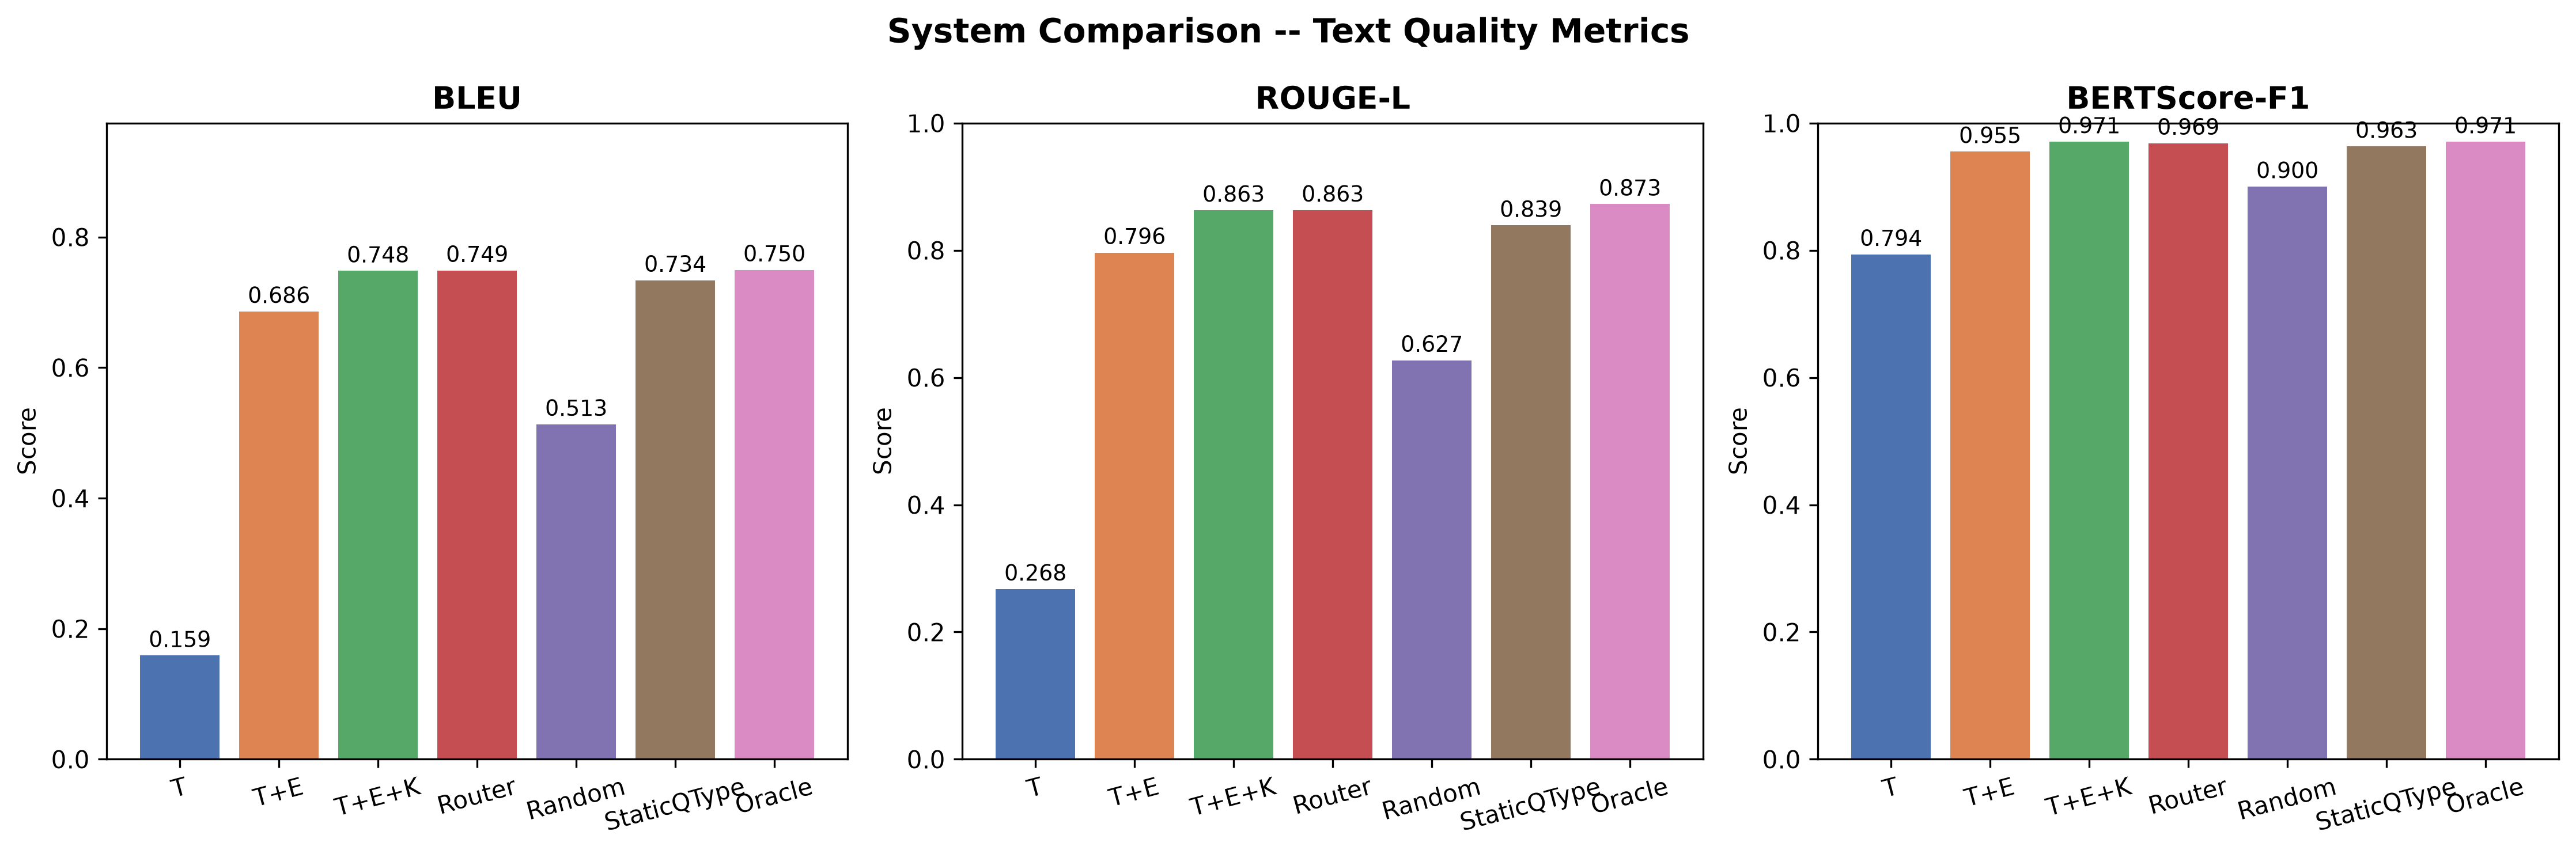
\includegraphics[width=\columnwidth]{summary_metrics.png}
\caption{Text-quality metrics across the seven evaluated systems ($n{=}300$).}
\label{fig:summary}
\end{figure}

\subsection{Router versus Always-On Hybrid Retrieval}

Table~\ref{tab:paired} reports paired differences on the same 300
questions. On all three quality metrics the difference between the
router and always-on hybrid retrieval is small and not statistically
detectable: BLEU $+0.0007$ ($p = 0.304$), ROUGE-L $+0.0002$
($p = 0.391$), and BERTScore~F1 $-0.0024$ ($p = 0.526$), with every
confidence interval straddling zero. The EHR-contradiction difference
is likewise not significant ($p = 0.157$).

Two differences are significant. Latency falls by 3522.8~ms, a 46.8\%
reduction ($p = 2.0\times10^{-42}$), achieved by invoking the KG on
only 52 of 300 questions (17.3\%); the router's overall mode
distribution is 174 T+E, 74 T, and 52 T+E+K, close to the oracle's
180, 73, and 47. The unsupported-claim rate, however, is
\textit{higher} for the router ($+0.0722$,
$p = 2.2\times10^{-10}$). Of the three pre-registered H1 criteria---
quality parity, a latency reduction of at least 25--40\%, and
hallucination no worse than always-on hybrid---the first two are met
and the third is not. Section~\ref{sec:grounding} examines whether
this reflects a measurement artifact.

\begin{table}[t]
\centering
\footnotesize
\setlength{\tabcolsep}{4pt}
\caption{Paired differences, Router $-$ T+E+K, on the same 300 questions. Intervals are 10{,}000-sample bootstrap; $p$-values are paired Wilcoxon.}
\label{tab:paired}
\begin{tabular}{lrrl}
\toprule
Metric & Diff. & 95\% CI & $p$ \\
\midrule
BLEU              & $+0.0007$ & $[-0.0009, +0.0022]$ & 0.304 \\
ROUGE-L           & $+0.0002$ & $[-0.0068, +0.0065]$ & 0.391 \\
BERTScore~F1      & $-0.0024$ & $[-0.0057, +0.0003]$ & 0.526 \\
EHR-contra.\      & $-0.0013$ & $[-0.0033, +0.0000]$ & 0.157 \\
Unsupported rate  & $+0.0722$ & $[+0.0517, +0.0949]$ & $2.2\times10^{-10}$ \\
Latency (ms)      & $-3522.8$ & $[-3705.7, -3330.0]$ & $2.0\times10^{-42}$ \\
\bottomrule
\end{tabular}
\end{table}

\subsection{Decomposing the Latency Advantage}

Table~\ref{tab:latency} separates retrieval from generation. Generation
cost is essentially constant across T+E, T+E+K, and the router
(3243.9, 3184.9, and 3182.6~ms), so the router's saving does not come
from shorter prompts or faster decoding. It comes entirely from
retrieval: knowledge-graph traversal accounts for 57.7\% of always-on
hybrid latency (4342.8~ms of 7527.7~ms), and the router reduces mean
retrieval cost to 822.3~ms by skipping it on most questions.

This also explains an apparent anomaly in Table~\ref{tab:main}: random
routing is slower than the router (4297.6~ms vs.\ 4004.9~ms) despite
much lower quality, because it invokes the KG more often (3.27 vs.\
2.04 mean retrieved facts).

\begin{table}[t]
\centering
\footnotesize
\setlength{\tabcolsep}{4pt}
\caption{Latency decomposition, mean milliseconds. Generation cost is near-constant; the router's advantage lies entirely in retrieval.}
\label{tab:latency}
\begin{tabular}{lrrrr}
\toprule
System & Retrieval & Generation & Total & Retr.~\% \\
\midrule
T           &   39.6 & 2170.0 & 2209.6 &  1.8 \\
T+E         &   97.4 & 3243.9 & 3341.3 &  2.9 \\
T+E+K       & 4342.8 & 3184.9 & 7527.7 & 57.7 \\
Router      &  822.3 & 3182.6 & 4004.9 & 20.5 \\
Random      & 1550.1 & 2747.5 & 4297.6 & 36.1 \\
StaticQType &  609.2 & 3180.8 & 3790.0 & 16.1 \\
Oracle      &  751.5 & 3210.2 & 3961.7 & 19.0 \\
\bottomrule
\end{tabular}
\end{table}

\subsection{What Drives Routing: Feature Ablation}
\label{sec:ablation}

The router was designed on the premise that patient state informs the
routing decision. We test that premise directly by retraining it on
feature subsets with identical hyperparameters
(Table~\ref{tab:ablation}).

The premise is not supported. A router using only the 384-dimensional
question embedding matches the full model's accuracy exactly (0.9200)
and achieves a \textit{higher} macro-F1 (0.8873 vs.\ 0.8692) and a
higher T+E+K F1 (0.8947 vs.\ 0.7895). Adding the five structural
patient features changes accuracy by $+0.0000$ and macro-F1 by
$-0.0181$. Patient features alone perform close to chance
(accuracy 0.3600).

The router nevertheless remains clearly better than static
alternatives: on the same validation split it reaches 0.9200 accuracy
against 0.8200 for both a question-type lookup and a stronger
exact-question-text lookup, and 0.5900 for the majority class. The
advantage over an exact-match lookup arises because embeddings
generalise to question phrasings unseen in training, on which a lookup
table has no entry at all. The correct characterisation is therefore a
learned question-driven routing policy, not a patient-adaptive one.

\begin{table}[t]
\centering
\footnotesize
\setlength{\tabcolsep}{4pt}
\caption{Router feature ablation on the validation split ($n{=}100$), identical hyperparameters throughout.}
\label{tab:ablation}
\begin{tabular}{lrrrr}
\toprule
Feature set & Dim. & Acc. & Macro-F1 & F1 T+E+K \\
\midrule
Majority class     &   0 & 0.5900 & 0.2474 & --- \\
Question embedding & 384 & 0.9200 & \textbf{0.8873} & \textbf{0.8947} \\
Patient features   &   5 & 0.3600 & 0.3385 & 0.2105 \\
Both (deployed)    & 389 & 0.9200 & 0.8692 & 0.7895 \\
\bottomrule
\end{tabular}
\end{table}

\subsection{Grounding under a Length-Controlled Measure}
\label{sec:grounding}

The unsupported-claim rate counts answer tokens absent from the
context, normalised by answer length. This falls mechanically as
context grows, so it penalises any system that retrieves less
independently of whether its answer is ungrounded. The confound is
large: pooled across systems, context length and unsupported rate
correlate at $r = -0.5169$ ($r^2 = 0.267$,
$p = 7.7\times10^{-144}$).

To remove it we score each answer twice, once against its real context
and once against a length-matched decoy context drawn from a different
question, and report the excess,
$\text{grounding} = \text{unsupported}_{\text{decoy}} -
\text{unsupported}_{\text{real}}$. Both terms carry the same length
bias, so it cancels; higher values indicate an answer better explained
by its own evidence than by unrelated evidence of equal size.

Table~\ref{tab:grounding} reports the result, and it does not overturn
the H1 finding. The router remains significantly less grounded than
always-on hybrid retrieval (0.5379 vs.\ 0.6271,
$p = 1.2\times10^{-5}$). The efficiency-grounding trade-off is
therefore real rather than an artifact of the original metric: routing
roughly a quarter of questions to a weaker mode measurably reduces how
well answers are supported by their retrieved evidence.

The corrected measure also exposes a result the original metric
obscured. Text-only retrieval scores 0.0152, meaning its answers are
barely better explained by their own retrieved passages than by an
unrelated context of the same length. Under the original metric mode T
appeared merely worse (0.5813); under the length-controlled measure it
is close to entirely ungrounded. We note that the corrected measure is
length-\textit{controlled} rather than length-independent: a residual
correlation of $r = +0.33$ remains, part of which plausibly reflects
genuine grounding gains from additional context.

\begin{table}[t]
\centering
\footnotesize
\setlength{\tabcolsep}{4pt}
\caption{Grounding before and after length control. Higher grounding excess is better.}
\label{tab:grounding}
\begin{tabular}{lrrr}
\toprule
System & Unsupported & vs.\ decoy & Grounding excess \\
\midrule
T           & 0.6982 & 0.7134 & 0.0152 \\
T+E         & 0.3566 & 0.8405 & 0.4839 \\
T+E+K       & 0.1872 & 0.8143 & \textbf{0.6271} \\
Router      & 0.2748 & 0.8127 & 0.5379 \\
Random      & 0.4038 & 0.7533 & 0.3495 \\
StaticQType & 0.3022 & 0.8063 & 0.5041 \\
Oracle      & 0.2802 & 0.8097 & 0.5295 \\
\bottomrule
\end{tabular}
\end{table}

\subsection{Retrieval Benefit across EHR Sparsity}

H2 predicted that knowledge-graph augmentation would matter more as
the structured record thins. The held-out data show the opposite
(Fig.~\ref{fig:sparsity}). The BERTScore~F1 advantage of T+E+K over
T+E is $+0.0195$ in low-sparsity admissions ($n = 169$), $+0.0120$ in
medium ($n = 101$), and only $+0.0057$ in high-sparsity admissions
($n = 30$). The ordering is monotonic and inverted relative to the
hypothesis.

Fig.~\ref{fig:routing} shows the router's mode choices by sparsity
bucket. We caution that the high-sparsity bucket contains only 30
questions, so the smallest of these gaps is the least precisely
estimated.

\begin{figure}[t]
\centering
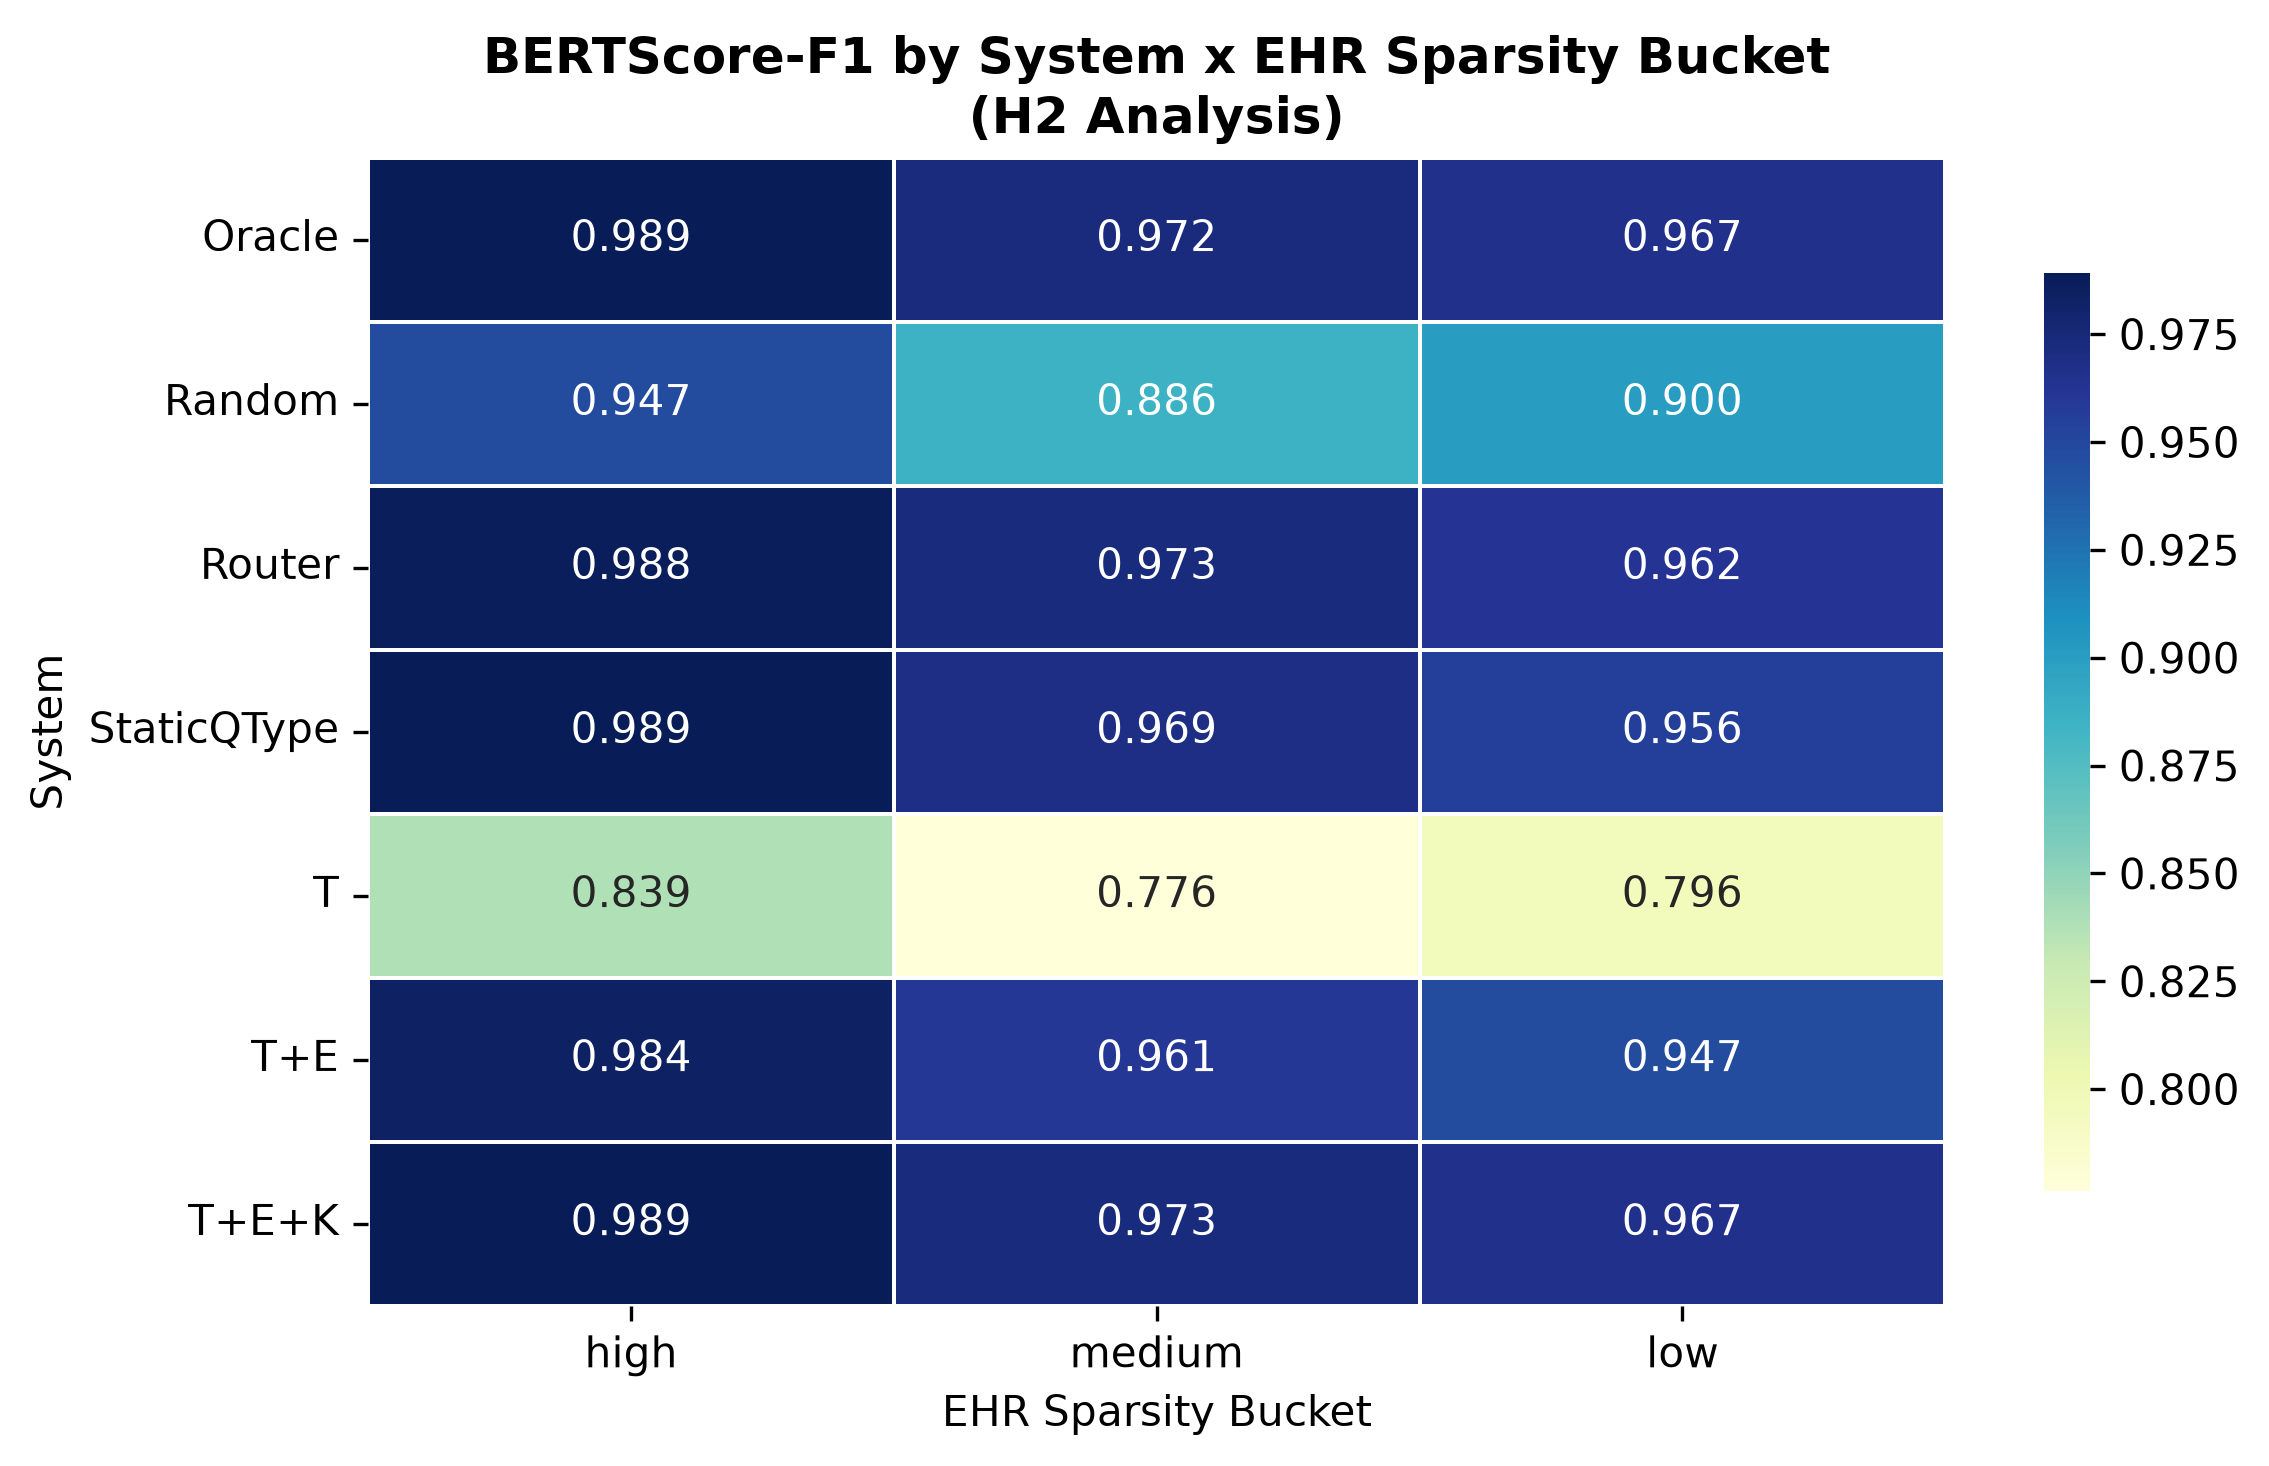
\includegraphics[width=\columnwidth]{sparsity_heatmap_bertscore_f1.png}
\caption{BERTScore~F1 by system and EHR sparsity bucket. The T+E+K advantage over T+E shrinks as sparsity increases.}
\label{fig:sparsity}
\end{figure}

\begin{figure}[t]
\centering
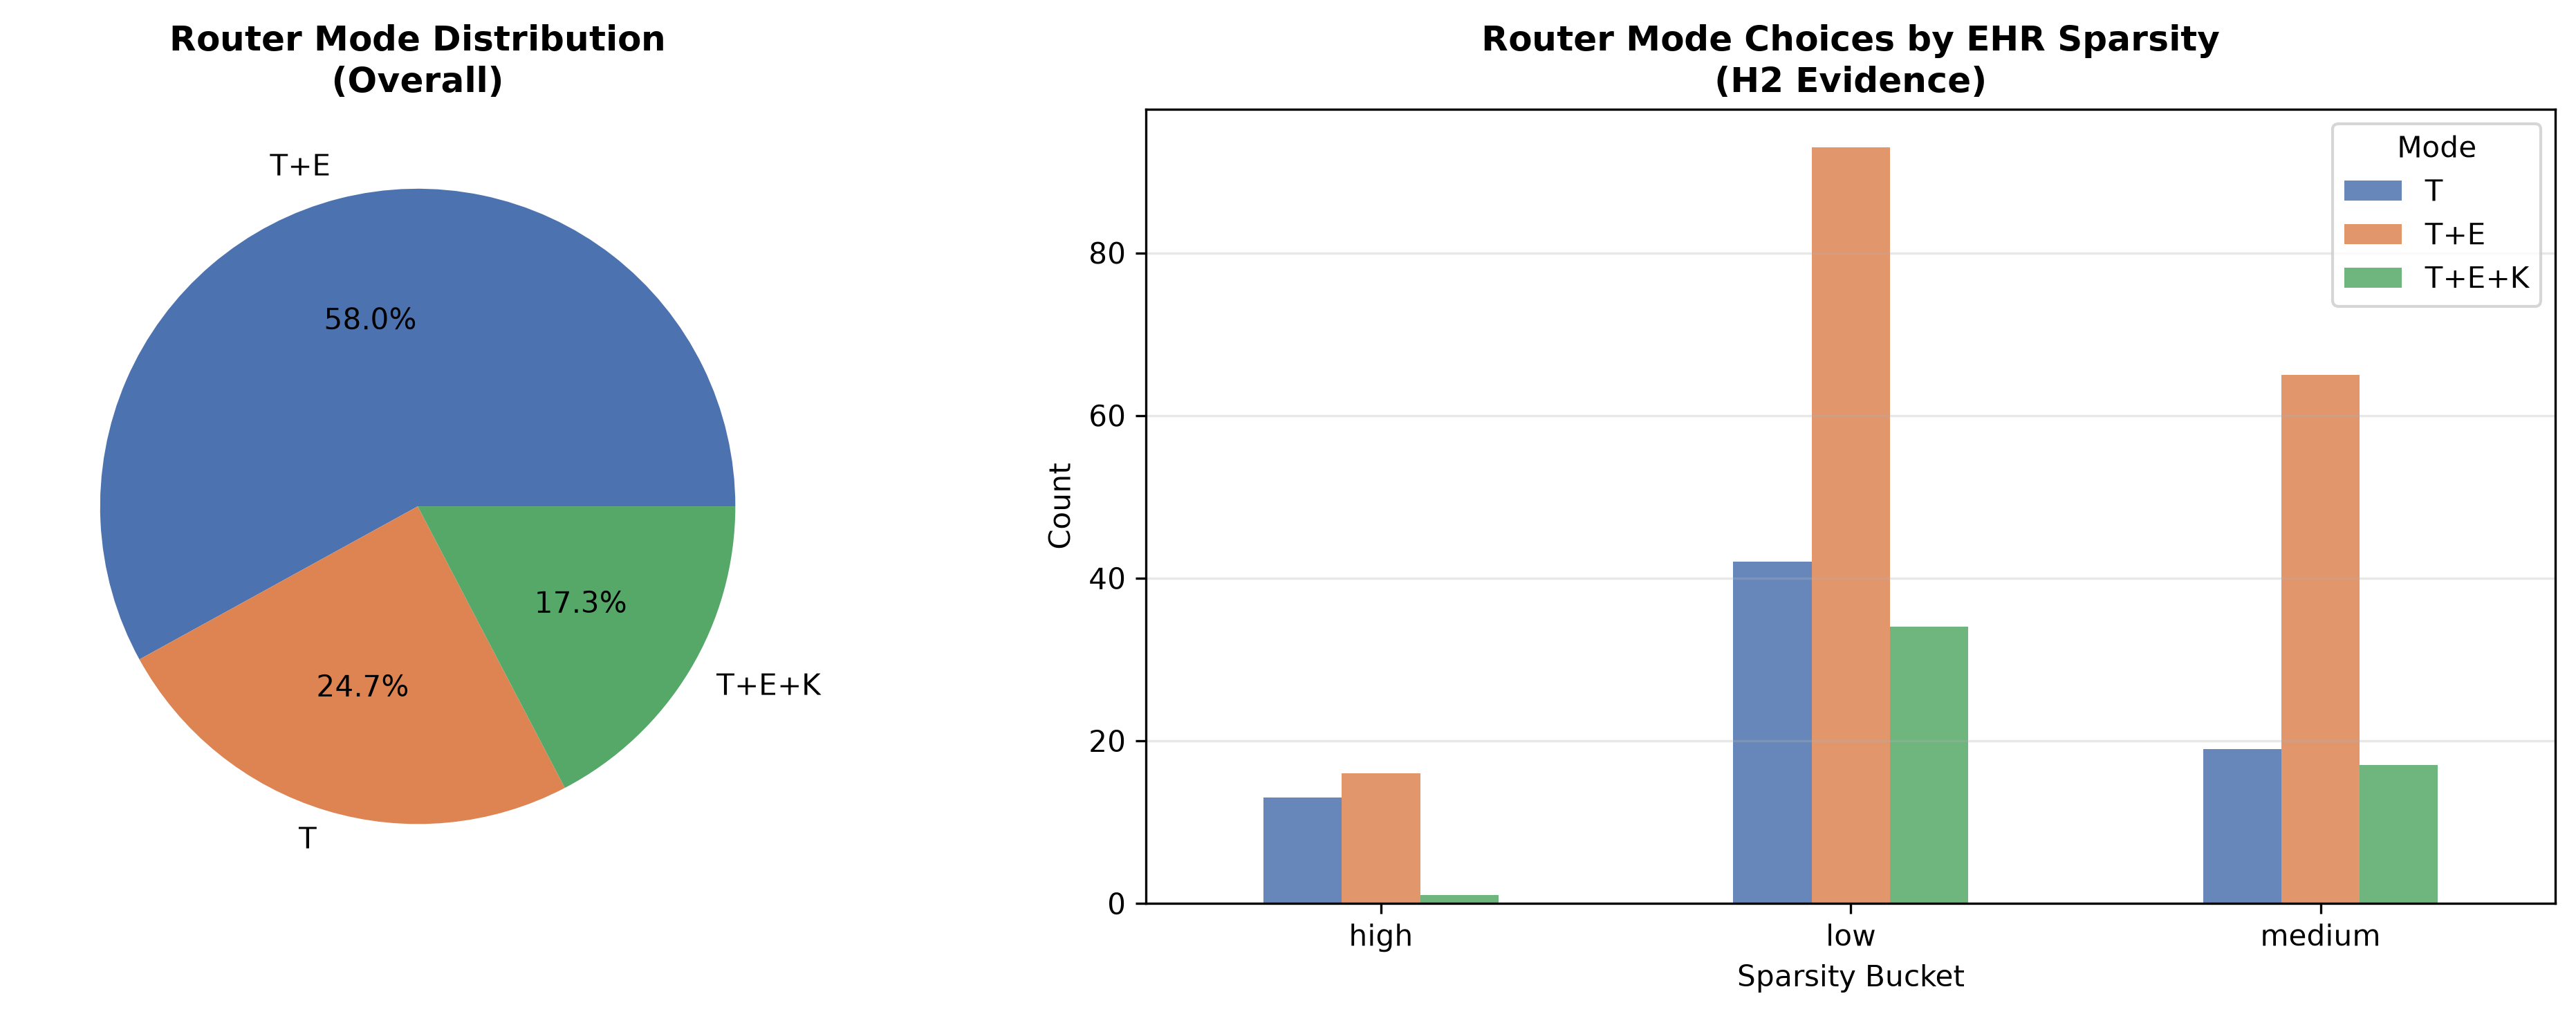
\includegraphics[width=\columnwidth]{router_mode_distribution.png}
\caption{Router mode selection overall and by EHR sparsity bucket.}
\label{fig:routing}
\end{figure}

\section{Discussion}

\subsection{Question-Driven, Not Patient-Adaptive, Routing}

The ablation in Section~\ref{sec:ablation} contradicts the premise
that motivated this system. Patient-level features add nothing, and
the routing decision is recoverable from the question alone. The
reason is visible in the task structure: for the template question
types used here, the best retrieval mode is largely determined by what
the question asks for. Questions requesting a diagnosis or a
laboratory value are answered from the structured record, and
questions requiring guideline knowledge benefit from the graph, almost
regardless of which patient is involved.

This does not make the router useless---it still outperforms both
static lookups and captures nearly all the oracle-available
headroom---but it narrows the claim. Adaptive retrieval in this
setting is a question-classification problem. Demonstrating genuinely
patient-adaptive routing would require a benchmark in which the same
question demands different evidence for different patients far more
often than ours does, a property our template-generated questions
largely lack (Section~\ref{sec:limitations}). We regard establishing
that this is testable, and that our benchmark does not test it, as a
useful negative result.

\subsection{Why Knowledge-Graph Benefit Shrinks under Sparsity}

The inverted H2 result has a concrete mechanism rather than being
noise. Our KG retrieval is keyed on the patient's diagnosis list:
diseases are matched from diagnosis strings, and the one-hop
neighbourhood of those matches is what enters the prompt. High EHR
sparsity is defined in part by having fewer than three distinct
diagnoses. Sparse records therefore supply fewer entry points into the
graph and retrieve fewer facts, exactly when the hypothesis predicted
the graph would matter most. The knowledge graph cannot fill a gap
when the gap includes its own index key.

This suggests the hypothesis was under-specified rather than simply
wrong. A KG retrieval strategy keyed on something a sparse record still
provides---presenting symptoms, ordered medications, or the question
itself---might show the predicted pattern. Our finding constrains the
claim to diagnosis-keyed graph retrieval.

\subsection{Implications for Grounding Metrics}

Word-overlap grounding metrics are widely used because they are cheap
and reference-free, but Section~\ref{sec:grounding} shows that in a
comparison across systems with different context sizes they measure
context length as much as grounding, with roughly a quarter of the
variance attributable to length alone. Any evaluation that compares
retrieval configurations of unequal size is exposed to this bias, and
it acts systematically against the more efficient system. The
decoy-context control we use is inexpensive, requires no additional
model, and reverses none of our conclusions---which is precisely why
it is worth applying: it converts an objection a reviewer would
otherwise raise into a tested and reported result.

\section{Limitations}
\label{sec:limitations}

The most consequential limitation is that our questions are
template-generated from structured EHR fields rather than authored by
clinicians. For several question types the gold answer is a field that
also appears verbatim in the T+E and T+E+K contexts, which inflates
absolute lexical scores; mode T, which lacks the EHR snapshot, scores
BLEU 0.1588, consistent with this explanation. Our findings therefore
speak to retrieval routing over structured-field questions, not to
open-ended clinical inquiry.

The scale is modest: 300 held-out questions over 61 admissions, a
single random seed, a single base model, and a single dataset. We
report bootstrap confidence intervals throughout, but we do not
estimate seed-to-seed or model-to-model variance, and the
high-sparsity subgroup contains only 30 questions.

The knowledge graph is small---25 diseases and 215 guideline
edges---and hand-curated rather than extracted from a standard
biomedical ontology, so coverage limits how often graph facts can
apply at all.

Our hallucination measures are automatic heuristics, not
clinician-adjudicated annotations, and we perform no human
evaluation and no inter-annotator agreement study. As reported, the
EHR-contradiction detector is structurally inapplicable to mode T.
Finally, we do not implement a KG-contradiction measure, so we cannot
say whether injected graph facts are themselves respected.

\section{Ethics and Responsible Use}

This work uses MIMIC-IV~\cite{mimiciv2023}, a de-identified critical
care dataset available under credentialed access requiring completion
of human-subjects research training and acceptance of a data use
agreement. No protected health information appears in this paper, and
no patient-level data, derived snapshots, retrieval indices, or
generated answers are released, and the fine-tuned generator adapter is
withheld because it was trained directly on patient-derived text. The
released artifacts are the source code, the hand-curated
guideline-derived knowledge-graph edges, the patient-identifier split
file (integer subject identifiers only, no clinical content), and the
trained router, a gradient-boosted tree over question embeddings and
five aggregate record counts that stores no patient text.

The system is a research prototype. It has not been validated
clinically, evaluated prospectively, or reviewed by clinicians for
safety, and it must not be used to inform patient care. Two results
here bear directly on that caution: text-only retrieval is close to
entirely ungrounded under our length-controlled measure, and the
efficiency gain from adaptive routing comes at a measurable cost in
answer grounding. Deployments that optimise for latency should
therefore expect a grounding penalty and evaluate it explicitly rather
than assume parity from aggregate quality scores.

\section{Conclusion}

We evaluated whether a learned router over three retrieval
configurations can reduce the cost of hybrid clinical RAG without
sacrificing answer quality. On 300 held-out questions from disjoint
patients, the router matched always-on hybrid retrieval on BLEU,
ROUGE-L, and BERTScore~F1 with no statistically detectable difference
while reducing latency by 46.8\%, and it outperformed random routing,
a static question-type policy, and an exact-question lookup.

Two pre-registered expectations failed, and we consider them the more
informative outcomes. A feature ablation showed that patient-level
features contribute no measurable routing signal, so the system is a
question-driven policy rather than the patient-adaptive one it was
designed to be. Under a length-controlled grounding measure the
router's grounding deficit persisted, establishing a real
efficiency-grounding trade-off rather than a metric artifact. Contrary
to hypothesis, knowledge-graph benefit decreased as EHR sparsity
increased, because graph retrieval keyed on the diagnosis list finds
fewer entry points in exactly the records that are sparse.

Taken together, the results support a narrower claim than the one we
set out to test: for structured-field clinical questions, retrieval
mode is largely predictable from the question, and skipping
knowledge-graph traversal on most questions is close to free in
quality but not in grounding.

\begin{thebibliography}{00}

\bibitem{thirunavukarasu2023} A.~J.~Thirunavukarasu, D.~S.~J.~Ting, K.~Elangovan, L.~Gutierrez, T.~F.~Tan, and D.~S.~W.~Ting, ``Large language models in medicine,'' \textit{Nature Medicine}, vol.~29, no.~8, pp.~1930--1940, 2023.

\bibitem{medgemma2025} A.~Sellergren \textit{et al.}, ``MedGemma technical report,'' \textit{arXiv preprint arXiv:2507.05201}, 2025.

\bibitem{lewis2020} P.~Lewis \textit{et al.}, ``Retrieval-augmented generation for knowledge-intensive NLP tasks,'' in \textit{Proc. NeurIPS}, 2020.

\bibitem{reimers2019} N.~Reimers and I.~Gurevych, ``Sentence-BERT: Sentence embeddings using Siamese BERT-networks,'' in \textit{Proc. EMNLP-IJCNLP}, 2019, pp.~3982--3992.

\bibitem{johnson2019} J.~Johnson, M.~Douze, and H.~J\'egou, ``Billion-scale similarity search with GPUs,'' \textit{IEEE Trans. Big Data}, vol.~7, no.~3, pp.~535--547, 2019.

\bibitem{xiong2024} G.~Xiong, Q.~Jin, Z.~Lu, and A.~Zhang, ``Benchmarking retrieval-augmented generation for medicine,'' in \textit{Findings of the Association for Computational Linguistics: ACL 2024}, 2024.

\bibitem{edge2024} D.~Edge \textit{et al.}, ``From local to global: A graph RAG approach to query-focused summarization,'' \textit{arXiv preprint arXiv:2404.16130}, 2024.

\bibitem{asai2024} A.~Asai, Z.~Wu, Y.~Wang, A.~Sil, and H.~Hajishirzi, ``Self-RAG: Learning to retrieve, generate, and critique through self-reflection,'' in \textit{Proc. ICLR}, 2024.

\bibitem{jeong2024} S.~Jeong, J.~Baek, S.~Cho, S.~J.~Hwang, and J.~C.~Park, ``Adaptive-RAG: Learning to adapt retrieval-augmented large language models through question complexity,'' in \textit{Proc. NAACL-HLT}, 2024.

\bibitem{mimiciv2023} A.~E.~W. Johnson, L.~Bulgarelli, L.~Shen \textit{et al.}, ``MIMIC-IV, a freely accessible electronic health record dataset,'' \textit{Scientific Data}, vol.~10, art.~1, 2023, doi:10.1038/s41597-022-01899-x.

\bibitem{duckdb2019} M.~Raasveldt and H.~M\"uhleisen, ``DuckDB: An embeddable analytical database,'' in \textit{Proc. ACM SIGMOD}, 2019, pp.~1981--1984.

\bibitem{bge2024} S.~Xiao, Z.~Liu, P.~Zhang, N.~Muennighoff, D.~Lian, and J.-Y.~Nie, ``C-Pack: Packed resources for general Chinese embeddings,'' in \textit{Proc. ACM SIGIR}, 2024.

\bibitem{dettmers2023} T.~Dettmers, A.~Pagnoni, A.~Holtzman, and L.~Zettlemoyer, ``QLoRA: Efficient finetuning of quantized LLMs,'' in \textit{Proc. NeurIPS}, 2023.

\bibitem{hu2022} E.~J.~Hu \textit{et al.}, ``LoRA: Low-rank adaptation of large language models,'' in \textit{Proc. ICLR}, 2022.

\bibitem{zhang2020} T.~Zhang, V.~Kishore, F.~Wu, K.~Q.~Weinberger, and Y.~Artzi, ``BERTScore: Evaluating text generation with BERT,'' in \textit{Proc. ICLR}, 2020.

\bibitem{lin2004} C.-Y.~Lin, ``ROUGE: A package for automatic evaluation of summaries,'' in \textit{Text Summarization Branches Out}, 2004, pp.~74--81.

\bibitem{chen2016} T.~Chen and C.~Guestrin, ``XGBoost: A scalable tree boosting system,'' in \textit{Proc. ACM SIGKDD}, 2016, pp.~785--794.

\bibitem{papineni2002} K.~Papineni, S.~Roukos, T.~Ward, and W.-J.~Zhu, ``BLEU: A method for automatic evaluation of machine translation,'' in \textit{Proc. ACL}, 2002, pp.~311--318.

\end{thebibliography}

\end{document}
